\documentclass[10pt]{beamer}

\usepackage[utf8]{inputenc}
\usepackage[T1]{fontenc}
\def\magyarOptions{frenchspacing=yes,refstruc=yes}
\def\bfdefault{b}

\usepackage[english,magyar]{babel}
\usepackage{graphics,epstopdf}
\usepackage{amsmath,amsfonts,amssymb,commath,bm}
\usepackage{ifthen}
\usepackage{helvet}
\usepackage{multicol}
\usepackage{multirow}
\usepackage{hyperref}
\usepackage[T1]{fontenc}
\usepackage{textcomp}
\usepackage{eurosym}
\usepackage{rotating}
\usetheme{ptektk}
\usepackage{xfrac}
\usepackage{wasysym}
\usepackage{listings}

\linespread{1.15}

\usecolortheme{orchid}
\useinnertheme{default}

\DeclareMathOperator*{\argmax}{arg\,max}
\DeclareMathOperator*{\argmin}{arg\,min}
\DeclareMathOperator{\Cov}{Cov}

\setlength{\parskip}{1ex}

\newcommand{\ind}{\perp\!\!\!\perp}
\newcommand*{\e}{\ensuremath{\mathrm{e}}}
\newcommand*{\T}{\ensuremath{\mathrm{T}}}
\newcommand*{\im}{\ensuremath{\mathrm{i}}}
\newcommand*{\sgn}{\ensuremath{\mathrm{sgn}}}
\newcommand*{\lin}{\ensuremath{\mathrm{lin}}}
\renewcommand*{\Re}{\ensuremath{\mathrm{Re}}}
\renewcommand*{\Im}{\ensuremath{\mathrm{Im}}}
\newcommand*{\E}{\ensuremath{\mathbf{E}}}
\renewcommand*{\P}{\ensuremath{\mathbf{P}}}

\newcommand{\bi}{\begin{itemize}}
\newcommand{\ei}{\end{itemize}}
\newcommand{\be}{\begin{enumerate}}
\newcommand{\ee}{\end{enumerate}}
\newcommand{\graybox}[1]{
	\par
	\fcolorbox{black}[rgb]{0.8,0.8,0.8}{
		\parbox{0.96\textwidth}{
			\vspace{0.5ex}
			\centering\parbox{0.93\textwidth}{
				#1
				}
			\vspace{0.5ex}
			}
		}
	\par
	}
	
\newcommand{\mybox}[1]{
	\par
	\fcolorbox{black}[rgb]{0.8,0.8,0.8}{
		\parbox{0.96\textwidth}{
			\vspace{0.5ex}
			\centering\parbox{0.93\textwidth}{
				#1
				}
			\vspace{0.5ex}
			}
		}
	\par
	}

\newtheorem{theo}{Tétel}
\newtheorem{lem}{Lemma}
\newtheorem{defi}{Definíció}

\title{Introduction to R}
\author{Herczeg Róbert, Kehl Dániel}
\institute{University of Pécs}
\date{2017/2018 ősz}

\begin{document}
\setbeamertemplate{background canvas}{
\includegraphics[width=\paperwidth]{ktk_title}}
\begin{frame}
\titlepage
\end{frame}
\setbeamertemplate{background canvas}{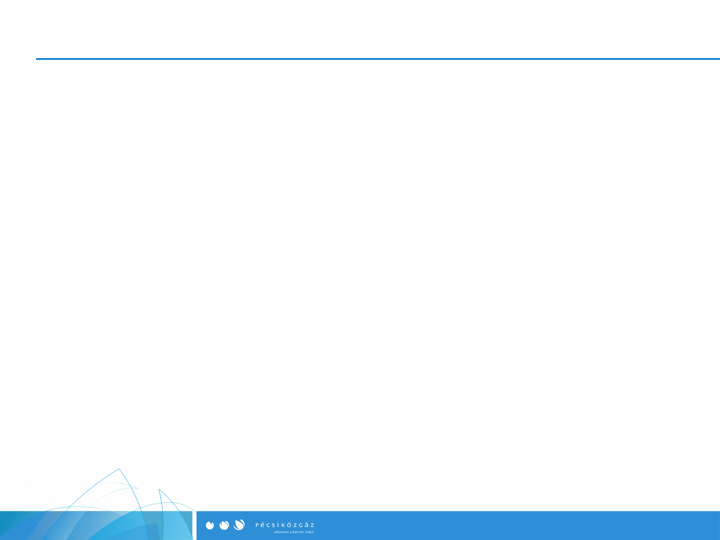
\includegraphics[width=\paperwidth]{ktk_slide}}

\begin{frame}{Motivation}
\begin{itemize}
\item R is used all over the world in many fields
\begin{itemize}
\item social sciences
\item econometrics
\item bioinformatics: \textcolor{blue}{\url{http://www.bioconductor.org}}
\item $\dots$
\end{itemize}
\item it is free, open source
\item user contributions are possible, and great advantage
\item one of the most enthusiastic user group (r-help mailing list)
\item a lot of great books (R series of Wiley, UseR!)
\item both in (reproducible) research and teaching
\item and here is a long story (maybe a little biased): \textcolor{blue}{\url{http://r4stats.com/articles/popularity}}

\end{itemize}
\end{frame}

\begin{frame}{Table of contents}
\tableofcontents
\end{frame}

\section{R basics}

\begin{frame}{R basics}
\framesubtitle{About the Project}
\begin{itemize}
\item \textcolor{blue}{\url{http://www.r-project.org}}
\item developed from the S language
\item free
\item consists of so called packages
\begin{itemize}
\item there are some basic packages (you have these after installing R)
\item you can find others (over 12350) on CRAN (The \textcolor{red}{C}omprehensive \textcolor{red}{R} \textcolor{red}{A}rchive \textcolor{red}{N}etwork) -- topic views
\item other user-provided functions and packages online
\end{itemize}
\item also very popular in academics
\end{itemize}
\end{frame}

\begin{frame}{R basics}
\framesubtitle{Pros and cons}
\begin{itemize}
\item you can basically find all (statistical) methods you might need
\item produces high quality, customizable, publication ready graphs
\item cooperates with other software packages (Excel, EViews, BUGS)
\item freedom
\item helps reproducible research
\item script language (limited GUI and point-and-click functionality)
\item running an analysis usually does not end with some tables and graphs (like in other software) but with objects containing information (and you can of course plot those or save them)
\end{itemize}
\end{frame}

\begin{frame}{R basics}
\framesubtitle{R Studio}
\begin{itemize}
\item a popular IDE (integrated development environment)
\item free, handy, convenient to use
\item ,,Matlab like''
\item you can download it at \textcolor{blue}{\url{https://www.rstudio.com/ide/download/}}
\item and here are some nice screenshots \textcolor{blue}{\url{https://www.rstudio.com/ide/screenshots/}}
\item we are going to use it on this short workshop
\end{itemize}
\end{frame}

\begin{frame}{R basics}
\framesubtitle{Basic functionality}
\begin{itemize}
\item prompt: > - waiting for input
\item try demo(), packages usually have demos, demo(persp), demo(graphics), demo(plotmath), demo(colors) etc.
\item use it as a calculator, simple operators and functions
\item define scalar variables: x = 1, x <- 1, 1 -> x (case sensitive!!!)
\item access history by up and down arrows
\item \# indicates a comment in the code
\item take a look at Appendix A (A sample session) in the R-intro.pdf!
\end{itemize}
\end{frame}

\begin{frame}{R basics}
\framesubtitle{Asking for help}
\begin{itemize}
\item ?functionname or help(functionname)
\begin{itemize}
\item first help pages might seem messy and too compicated, you have to get used to it, after some (a lot in fact) experience they are easy too use, informative and well structured
\item go for the examples if nothing else works (example(functionname))
\end{itemize}
\item help(''char'') and ?''char'' work in case of some special characters
\item ?packagename
\item help.start()
\item help.search() or ??
\item R-intro.pdf comes with R
\item www, google, \textcolor{blue}{\url{http://stats.stackexchange.com}}
\item if no result, ask your question on the r-help mailing list
\begin{itemize}
\item please read \textcolor{blue}{\url{http://www.r-project.org/posting-guide.html}}
\end{itemize}
\end{itemize}
\end{frame}

\begin{frame}{R basics}
\framesubtitle{Installing packages}
\begin{itemize}
\item install.packages(packagename)
\begin{itemize}
\item choose a mirror, this downloads the files needed from CRAN
\item you only have to do this once
\item try install.packages(''googleVis'')
\end{itemize}
\item library(packagename): activates the package (check library())
\begin{itemize}
\item now you can use the functions in the package
\item you have to do this every time you need the package
\item try library(,,googleVis'')
\end{itemize}
\item take a look at your new package with ?googleVis
\item try demo(WorldBank) and demo(AnimatedGeoMap), you probably have to wait a couple of seconds
\end{itemize}
\end{frame}

\section{Interactive graphs with Shiny}

\begin{frame}{Interactive graphs with Shiny}
\framesubtitle{Webscraping with Shiny}
\begin{itemize}
\item Collect semi-structured or unstructured data from websites
\begin{itemize}
\item install shiny, shinydashboard package - app
\item install rvest package for webscraping
\item googleVis is already installed
\end{itemize}
\item Develope a simple shiny app to visualize the data
\item Use interactive graph to show the data
\end{itemize}
\end{frame}

\begin{frame}{Interactive graphs with Shiny}
\framesubtitle{Webscraping - download data}
\begin{itemize}
\item Scraping data from web - ratebeer.com
\begin{itemize}
\item html, body, table, tr, td
\item load rvest package
\item rvest::read\_html - download webpage
\item rvest::html\_table - get tables from webpage
\item find the right table
\end{itemize}
\item data preprocessing
\end{itemize}
\end{frame}

\begin{frame}{Interactive graphs with Shiny}
\framesubtitle{Webscraping - Shiny, shinydashboard}
\begin{itemize}
\item easily create webapps with Shiny
\begin{itemize}
\item ui.R - user interface
\item server.R - server interface for the calculation
\item app.R - combine ui.R and server.R
\end{itemize}
\item shinydashboard
\begin{itemize}
\item increased UX - user experience
\item more options - sidebar, widgets, tabs etc.
\end{itemize}
\end{itemize}
\end{frame}

\section{Personalized midterms with the exams package}


\begin{frame}{Personalized exams}
\framesubtitle{Main challenges in big classes}
\begin{itemize}
\item high number of student especially on the Hungarian Programme
\begin{itemize}
\item high number of exams, takes a lot of time grading, creating new problems, datasets etc.
\item after midterms students want to check their exams, solutions etc.
\end{itemize}
\item desire to ,,force'' students to continuously follow the course material throughout the semester
\begin{itemize}
\item in-class short, 5 minute quizzes every lab session
\item two Excel-based midterms
\end{itemize}
\item exams at the computer makes cheating easier
\end{itemize}
One possible solution is personalized exams (with Moodle) and R.
\end{frame}

\begin{frame}{Personalized midterms}
\framesubtitle{Assessment structure of the semester}
\begin{center}
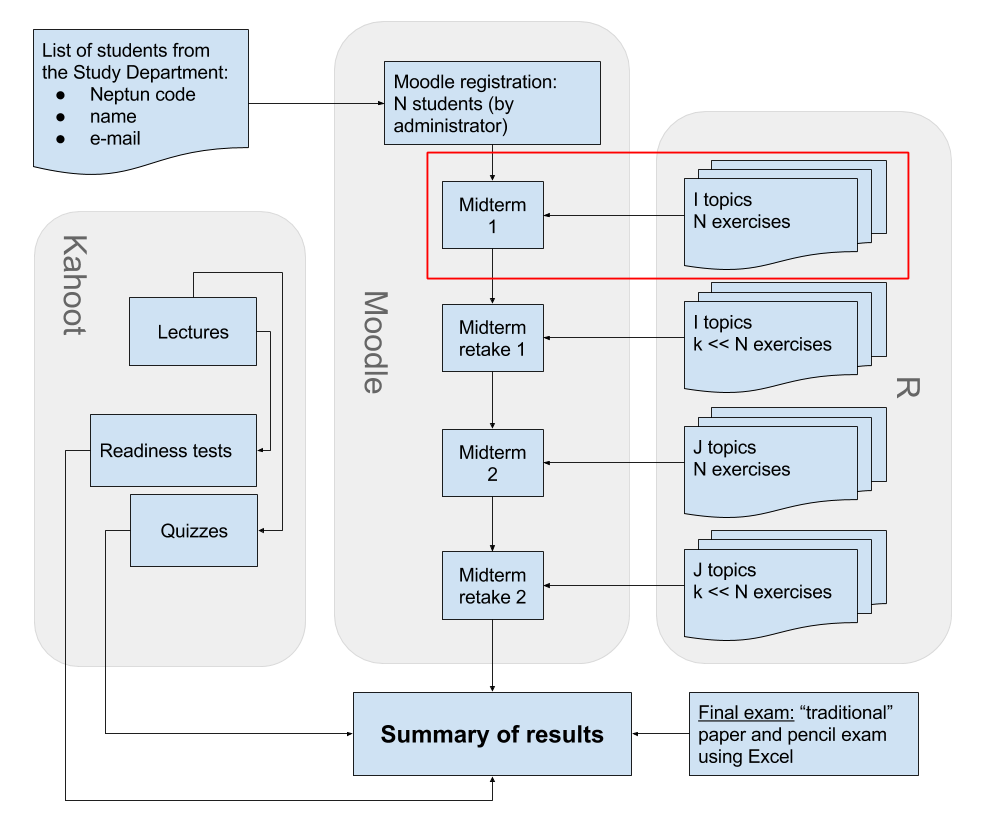
\includegraphics[scale = .25]{graph/semester_workflow_eng.png}
\end{center}
\end{frame}

\begin{frame}{Personalized midterms}
\framesubtitle{Storing exercise text and data in spreadsheets}
The example of estimation/hypothesis testing of the population mean
\begin{center}
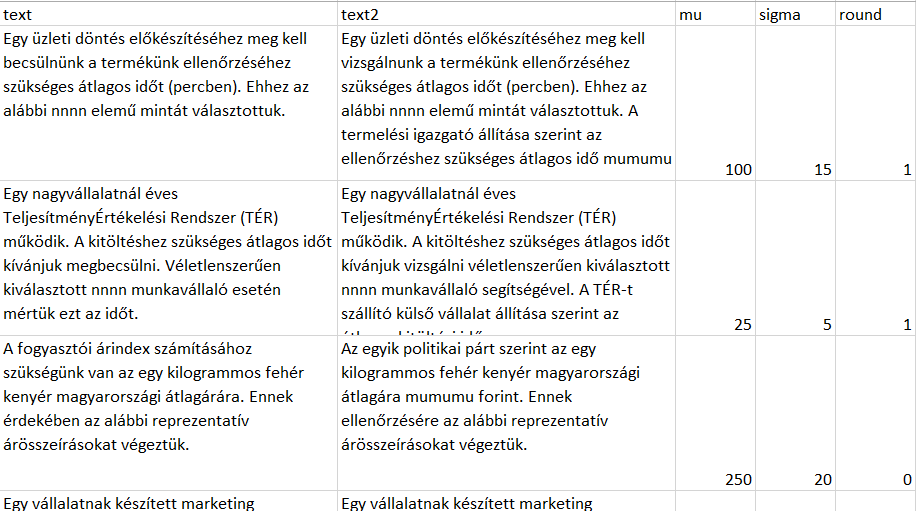
\includegraphics[width = \textwidth]{graph/excel.png}
\end{center}
\end{frame}

\begin{frame}{Personalized midterms}
\framesubtitle{The R-code -- generating data and solution}
\begin{center}
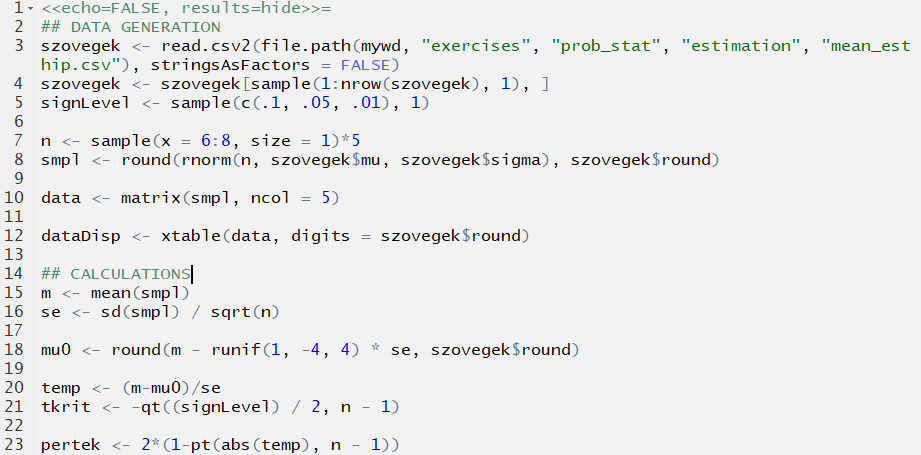
\includegraphics[width = \textwidth]{graph/R.png}
\end{center}
\end{frame}

\begin{frame}{Personalized midterms}
\framesubtitle{The R-code -- generating questions, setting tolerances}
\begin{center}
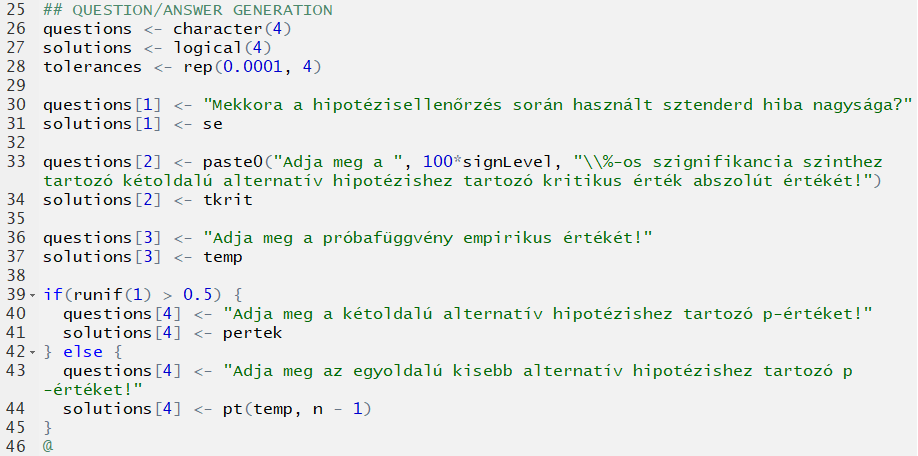
\includegraphics[width = \textwidth]{graph/R2.png}
\end{center}
\end{frame}

\begin{frame}{Personalized midterms}
\framesubtitle{Output in Moodle}
\begin{center}
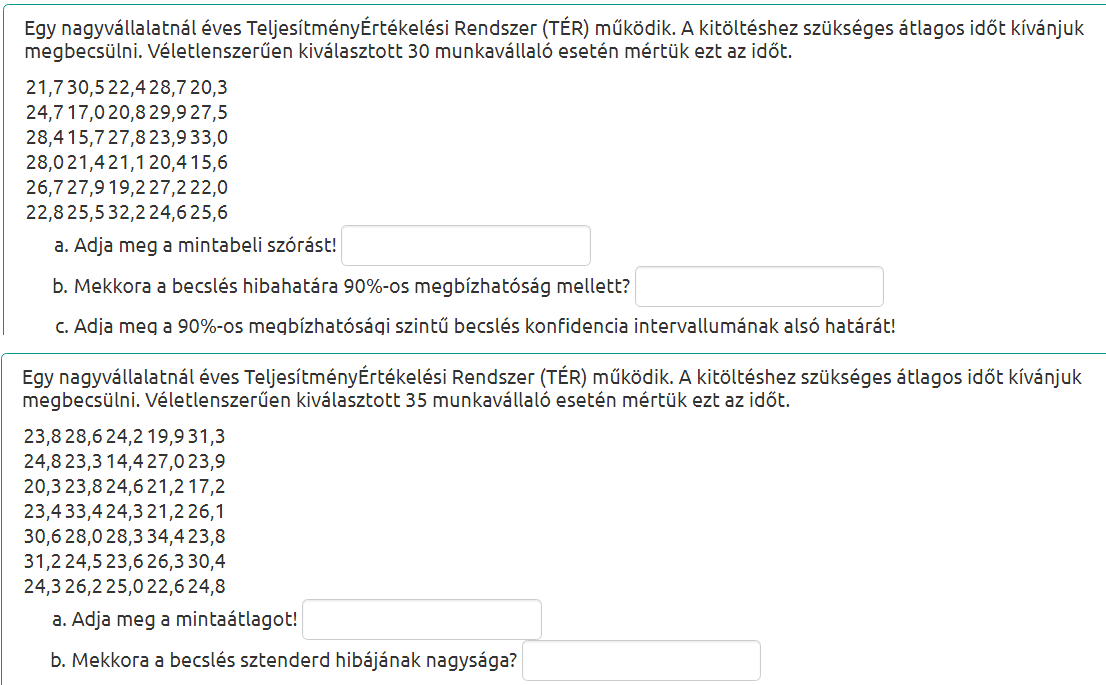
\includegraphics[scale=0.4]{graph/moodle.png}
\end{center}
\end{frame}

\begin{frame}{Personalized midterms}
\framesubtitle{The general idea -- workflow}
\begin{center}
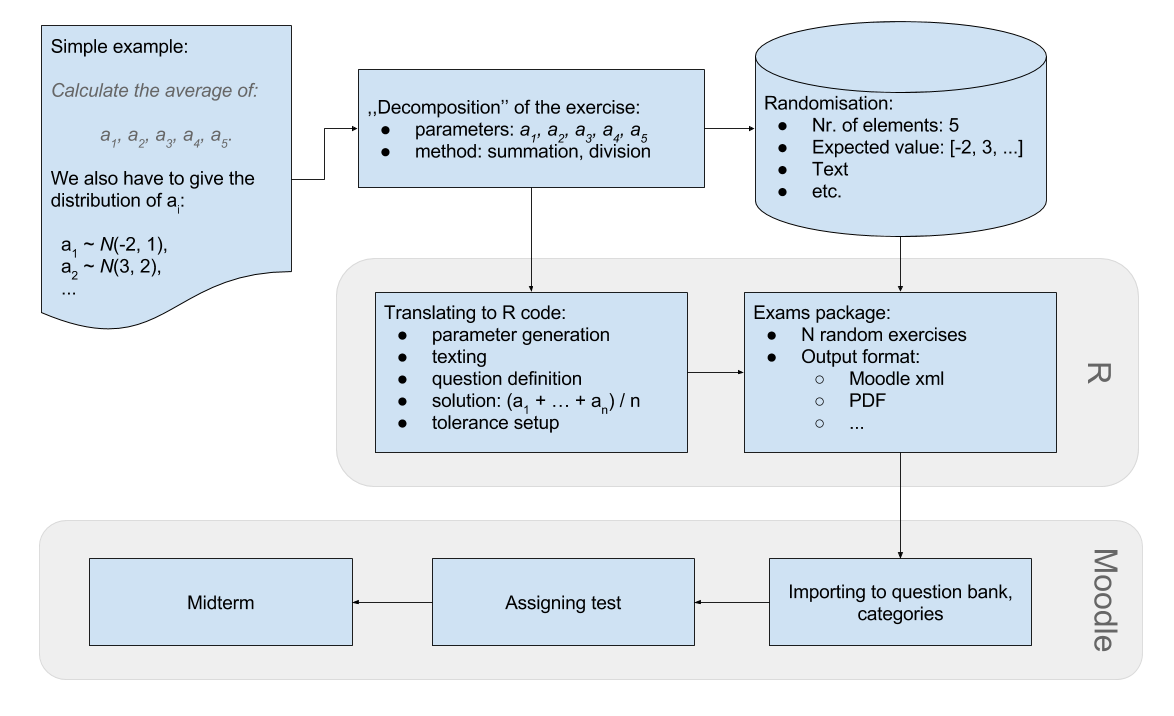
\includegraphics[width = \textwidth]{graph/zh_workflow_eng.png}
\end{center}
\end{frame}

\begin{frame}{Personalized midterms}
\framesubtitle{The R-code -- generating a midterm}
\begin{center}
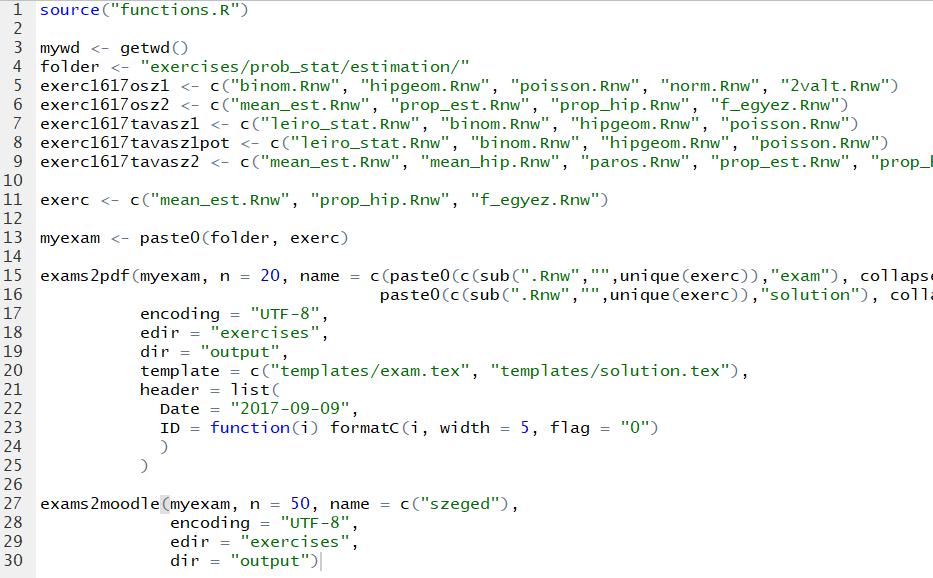
\includegraphics[width = \textwidth]{graph/R3.png}
\end{center}
\end{frame}

\begin{frame}{As a result}
\framesubtitle{our students face}
\begin{itemize}
\item very similar question types (let's say one-sample t-test, ANOVA, estimation and linear regression) \\ \textbf{BUT}
\item different ,,stories''
\item different questions (give the empirical value vs. give the critical value vs. give the p-value etc.)
\item different datasets
\item different numeric solutions
\item immediate feedback and results
\item possibility to ,,flag'' questions in Moodle
\end{itemize}
\end{frame}

\begin{frame}{Summary of our experiences}
\begin{itemize}
\item results are fairly similar in comparison to previous years
\item students do not complain about it, like the quick response
\item preparing a midterm takes longer (see R code)
\item setting up a question bank is an initial investment
\item going through flagged questions is fairly quick
\item saving a lot of time with automatic grading
\item cheating seems to be harder
\end{itemize}
\end{frame}

\begin{frame}{Useful links and materials}
\begin{itemize}
\item https://moodle.org/
\item R Core Team (2016). R: A language and environment for statistical computing. R Foundation for Statistical Computing,
  Vienna, Austria. URL https://www.R-project.org/.
\item Achim Zeileis, Nikolaus Umlauf, Friedrich Leisch (2014). Flexible Generation of E-Learning Exams in R: Moodle Quizzes,
  OLAT Assessments, and Beyond. Journal of Statistical Software 58(1), 1-36. doi:10.18637/jss.v058.i01
\item https://cran.r-project.org/web/packages/exams/vignettes/exams.pdf
\item https://cran.r-project.org/web/packages/exams/exams.pdf
\item exams\_skeleton function
\end{itemize}
\end{frame}


\end{document}